\section{Data Preprocessing}\label{data_preprocessing}

Data preprocessing is a vital step in the data mining process, particularly in the context of deep learning for image classification. This step involves techniques such as image augmentation, affine transformations, and resizing, which are essential for enhancing model performance. For this project, preprocessing is applied to the provided dataset (dataset\_19) to ensure it is suitable for the brain tumor classification task. The specific steps involved in the preprocessing of this dataset are outlined below.

\subsection{Image Cropping and Enhancement}\label{image_cropping_enhancement}

A fundamental step in our preprocessing workflow involves meticulous image cropping and enhancement to focus exclusively on the brain, thereby eliminating irrelevant background elements. This sequence of procedures ensures that the model concentrates on significant features, enhancing the effectiveness of the classification task. Below is a detailed outline of the improved process:

\subsubsection{Conversion and Blurring}

Initially, techniques adapted from previous research \cite{healthcare10091801} involve converting the images to grayscale. This conversion reduces computational complexity and highlights structural attributes by removing the color dimension. Subsequently, a Gaussian blur with a $3 \times 3$ kernel, as detailed in current solutions \cite{brainsci13091320}, is applied to the grayscale images. This blurring process effectively softens image noise, facilitating more reliable edge detection in the subsequent processing stages.

\subsubsection{Thresholding and Morphology}

The grayscale images are then subjected to adaptive thresholding, using a threshold value of 45 to convert them into binary images. This method, adapted from existing research \cite{Vimala_Srinivasan_Mathivanan_Mahalakshmi_Jayagopal_Dalu_2023}, effectively separates brain tissue from the background. The resulting binary images undergo a series of morphological operations, including two iterations each of erosion and dilation, to remove small noise regions and clarify the structural outline of the brain.

\subsubsection{Contour Detection and Cropping}

Using the thresholded images, contours are extracted with an external retrieval mode. The largest contour is presumed to delineate the brain's boundary. The extreme points of this contour (left, right, top, and bottom) are identified, and the image is cropped to a bounding rectangle that includes a configurable pixel margin to ensure the brain is isolated without being clipped as described in this study \cite{10.3389/fnhum.2023.1150120}. This precise cropping method ensures that only the brain region is retained for further processing \cite{Vimala_Srinivasan_Mathivanan_Mahalakshmi_Jayagopal_Dalu_2023}.

\subsubsection{Further Processing}

Each cropped image is first converted back to grayscale to focus on intensity variations, which are crucial for medical imaging. To enhance image quality, bilateral filtering is applied, which reduces noise while preserving important edge details, thus improving clarity and highlighting critical features. To further enhance visual contrast, the images are mapped to a 'bone' color scheme, which helps in better differentiation of structures.

Finally, the images are resized to dimensions that are optimal for each specific classification model. This resizing ensures uniformity within the dataset and maximizes computational efficiency by tailoring the pixel dimensions to the requirements of different models. This approach allows for the accommodation of varying input size specifications, ensuring that each model can effectively process the images without compromising performance or accuracy \cite{9926057}.

These steps, as implemented in our preprocessing workflow and illustrated in Figure \ref{fig:image_cropping}, significantly reduce computational load and enhance the clarity of critical features, which in turn improves the model's classification performance. This preprocessing method effectively prepares the dataset for further analysis, ensuring that the focus remains on the relevant anatomical structures necessary for accurate classification.

\begin{figure}[H]
  \centering
  \begin{subfigure}[b]{0.3\textwidth}
    \centering
    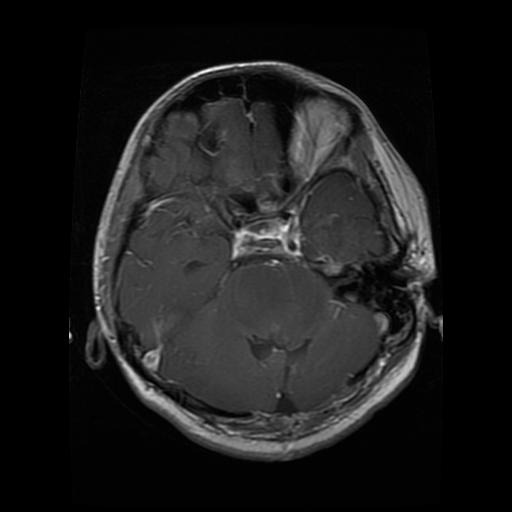
\includegraphics[width=\textwidth]{Exploration/Te-gl_0010.jpg}
    \caption{Original Image}
    \label{fig:original_image}
  \end{subfigure}
  \begin{subfigure}[b]{0.3\textwidth}
    \centering
    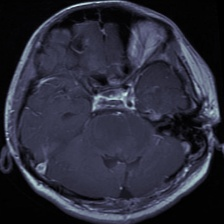
\includegraphics[width=\textwidth]{Exploration/Te-gl_0010_preprocessed.jpg}
    \caption{Preprocessed Image}
    \label{fig:preprocessed_image}
  \end{subfigure}
  \caption{Cropping the MRI image along its contour.}\label{fig:image_cropping}
\end{figure}


\subsection{Data Augmentation}\label{data_augmentation}

Following the initial preprocessing steps, we apply image augmentation techniques using the \texttt{ImageDataGenerator} class from the Keras library. Each model is fine-tuned with a subset of these techniques, which include horizontal flips, random rotations, and normalization. As referenced in \cite{nalepa_data_2019}, certain affine augmentations can be advantageous for brain tumor classification tasks. However, it is crucial to note that some augmentations, such as vertical flips, may be detrimental due to the potential misrepresentation of tumor locations.

Importantly, these augmentation techniques are applied exclusively to the training dataset, while the validation dataset remains unaltered. This strategy ensures that the model encounters a diverse array of augmented images during training, thereby enhancing its generalization capabilities without compromising the integrity of the evaluation process.

For each model evaluation, we provide a detailed commentary on the preprocessing and augmentation techniques employed, along with the rationale behind their selection. This comprehensive analysis elucidates how these techniques contribute to the overall performance and generalization capabilities of the models.

\subsection{Data Splitting}\label{data_splitting}
After preprocessing and augmentation, the dataset is divided into training and validation sets, with the training set comprising 80\% of the data and the validation set the remaining 20\%. This distribution allows the model to be trained extensively while also being evaluated on a separate set of data to assess its performance, as depicted in Figure \ref{fig:data_split}.

\begin{figure}[H]
  \begin{center}
    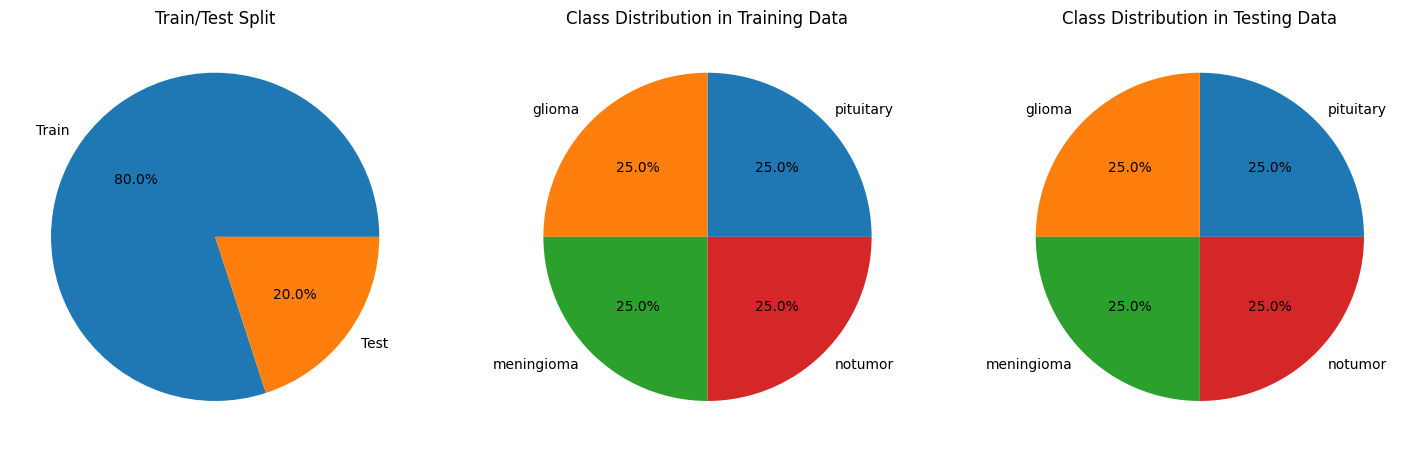
\includegraphics[width=0.95\textwidth]{Exploration/data_split.png}
  \end{center}
  \caption{Splitting the dataset into training and validation sets.}\label{fig:data_split}
\end{figure}


\subsection{Summary and Justifications}

\begin{figure}[H]
  \centering
  \begin{subfigure}[b]{0.4\textwidth}
    \centering
    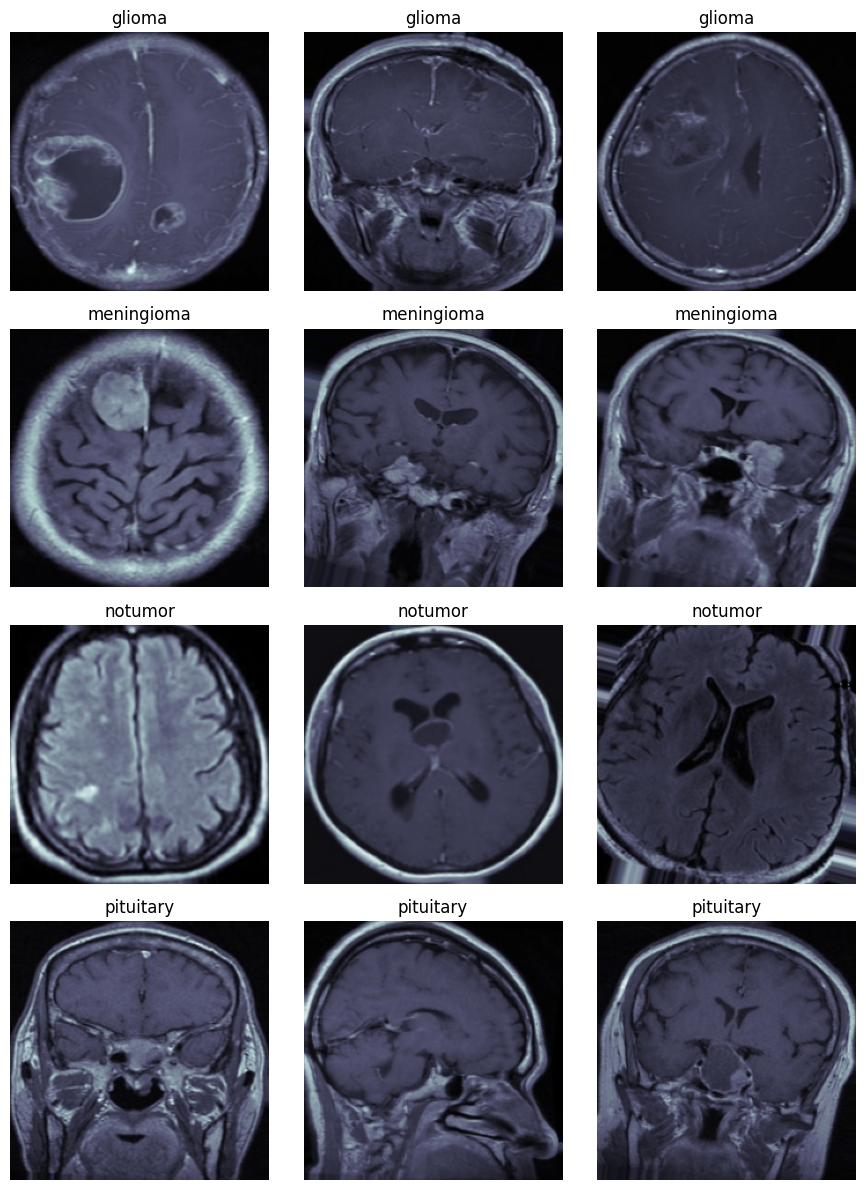
\includegraphics[width=\textwidth]{augmentation/train.png}
    \caption{Training Set}
    \label{fig:train_set}
  \end{subfigure}
  \hfill
  \begin{subfigure}[b]{0.4\textwidth}
    \centering
    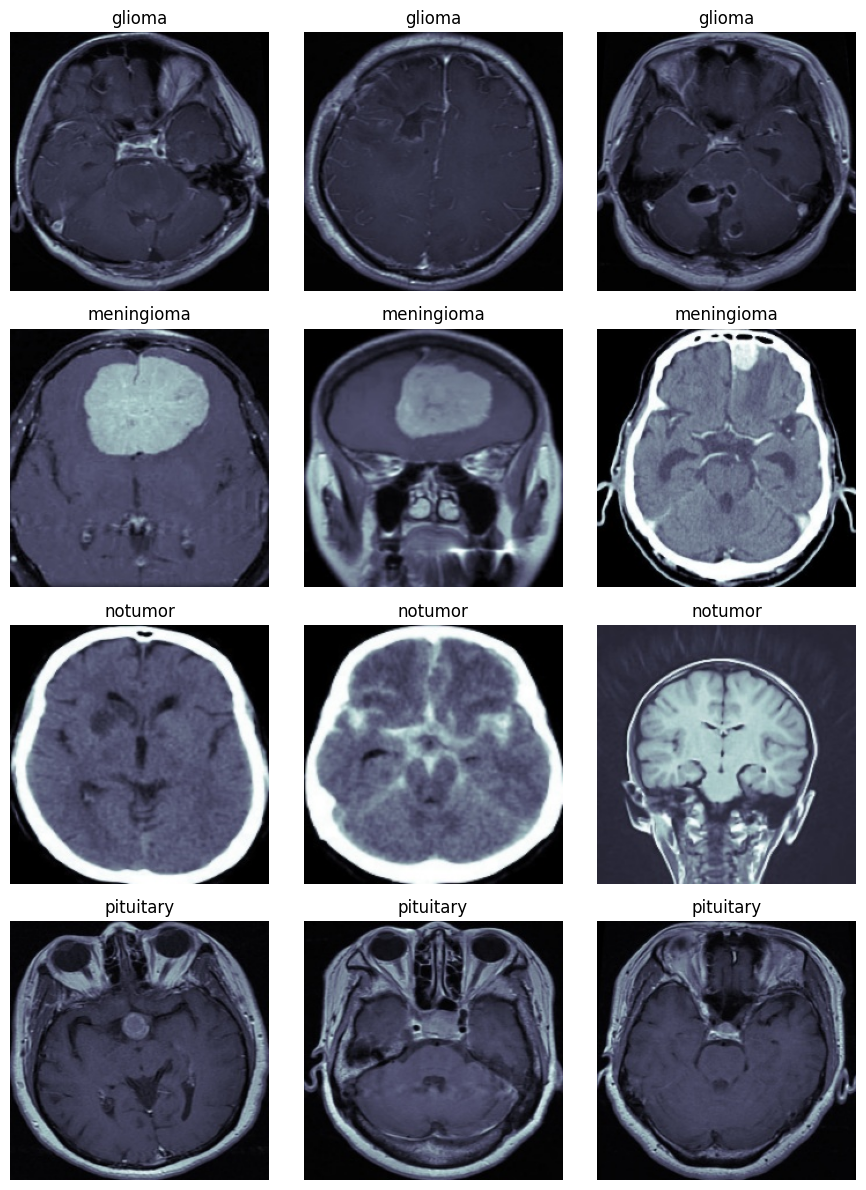
\includegraphics[width=\textwidth]{augmentation/test.png}
    \caption{Test Set}
    \label{fig:test_set}
  \end{subfigure}
  \caption{Tumor images in the training and test sets.}
  \label{fig:train_test_sets}
  
\end{figure}

Given the relatively small size of dataset\_19 (480 images in total), data augmentation is crucial for enhancing the dataset's variability and improving the model's generalization capabilities.

Training augmentation includes horizontal flipping, which is justified by the anatomical symmetry of the brain's hemispheres. This technique increases the diversity of the training data without misrepresenting tumor locations \cite{nalepa_data_2019}. This is particularly important given the limited size of the dataset compared to larger datasets, such as those used in the BraTS competition.

Testing augmentation involves random rotations, as brain images can be rotated in various directions. This further increases the dataset's variability and aids in model training. These augmentation strategies are essential for compensating for the smaller dataset size by exposing the model to a wider variety of image orientations and perspectives. This approach helps create a more robust model capable of accurately classifying brain tumors despite the limited amount of original training data.

The images in Figure \ref{fig:train_test_sets} show examples of the tumor images in the training and test sets after augmentation. The training set contains augmented images, while the test set remains unaltered. This ensures that the model is trained on a diverse range of images while being evaluated on a separate, unbiased dataset.
